\documentclass[tikz]{standalone}
\usepackage{tikz,amsmath}
\usetikzlibrary{calc}
\tikzstyle{vertex} = [draw, shape=circle, minimum width=.3cm, inner sep=.5pt]
\begin{document}
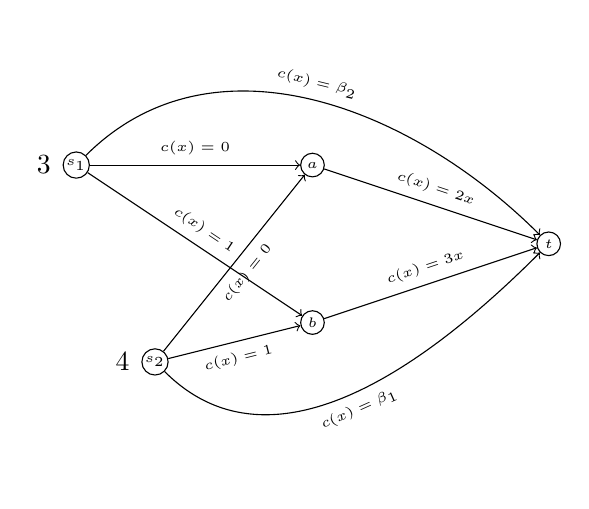
\begin{tikzpicture}[sloped]
    \draw (0,-.5) node[vertex] (s2) {\tiny{$s_2$}};
    \draw (-1,2) node[vertex] (s1) {\tiny{$s_1$}};
    \draw (2,0) node[vertex] (m2) {\tiny{$b$}};
    \draw (2,2) node[vertex] (m1) {\tiny{$a$}};
    \draw (5,1) node[vertex] (t) {\tiny{$t$}};
    \draw [->] (s1) -- node [above] {\tiny{$c(x)=0$}} (m1) ;
    \draw [->] (s1) -- node [above] {\tiny{$c(x)=1$}} (m2) ;
    \draw [->] (s2) -- node [below] {\tiny{$c(x)=0$}} (m1);
    \draw [->] (s2) -- node [below] {\tiny{$c(x)=1$}} (m2);
    \draw [->] (m1) -- node [above] {\tiny{$c(x)=2x$}}(t);
    \draw [->] (m2) -- node [above] {\tiny{$c(x)=3x$}}(t);
    \draw (s2) edge[out=-45,in=-135,->] node [below] {\tiny{$c(x)=\beta_1$}} (t);
    \draw (s1) edge[out=45,in=135,->] node [above] {\tiny{$c(x)=\beta_2$}} (t);
    \node at (s1) [left=.2cm] {$\tiny{3}$};
    \node at (s2) [left=.2cm] {$\tiny{4}$};
\end{tikzpicture}
\end{document}
